\documentclass[../all.tex]{subfiles}
\begin{document}
%%%%%%%%%%%%%%%%%%
    \section{Sports Fake Detector}
%%%%%%%%%%%%%%%%%%

\subsection{Tecnologías utilizadas}
    \subsubsection{MongoDB}
        MongoDB es un sistema de bases de datps NoSql de código abierto orientado a documentos. En lugar de almacenar la información en tablas como se haría en una base de datos relacional, MongoDB guarda la información en forma de documentos JSON, haciendo que la integración de este sistema de información sea mucho más simple y rápido que otros sistemas de bases de datos.\\
        MongoDB ha sido muy útil para almacenar de manera eficiente grandes conjuntos de tuits. Para trabajar con este sistema de bases de datos se ha empleado la líbreria PyMongo, que es la distribución para Python recomendada en la web oficial de MongoDB y que contiene todas las herramientas necesarias. Para el proyecto se ha empleado la versión 3.0.4 de MongoDB.\\
        MongoDB es un sistema fácil de utilizar y que funciona muy bien para guardar textos pero vamos a ver una tabla donde se puede comparar una base de datos como MongoDB con una SQL\footnote{Obtenida en \url{https://blog.pandorafms.org/es/bases-de-datos-nosql/}}.
        
    
        
        \begin{center}
            \begin{tabular}{ | m{3cm} | m{4cm}| m{4cm} | } 
                \hline
                \textbf{Feature} & \textbf{NoSQL Database} & \textbf{SQL Database} \\ 
                \hline
                Performance & High \checkmark & Low \\ 
                \hline
                Reliability & Poor & Good \checkmark \\ 
                \hline
                Availability & Good & Good \\ 
                \hline
                Consistency & Poor & Good \checkmark \\ 
                \hline
                Dara storage & Optimized for huge data \checkmark & Medium sized to large  \\ 
                \hline
                Scalability & High \checkmark & High but expensive  \\ 
                \hline
            \end{tabular}
        \end{center}
    \newpage
    \subsubsection{Pymongo 3.7.1}
        Pymongo es una librería de Python para poder conectarnos a una base de datos MongoDB.
        Para utilizar esta librería se utilizará una clase propia.
        \begin{figure}[H]
        	\centering
        	\includegraphics[height=13cm, width=15cm]{imgs/DB_class.png}
        	\caption{Clase DB utilizada para la comunicación entre el programa y la base de datos en MongoDB}
        \end{figure}
        
    \subsubsection{AVL Tree}
        
    	Todas las palabras están guardadas en una base de datos MongoDB pero con la finalidad de hacer la búsqueda más rápida una vez se consultan por primera vez se quedan guardadas en un árbol propio, concretamente en un AVL tree. \\
    	
    	Un árbol es un tipo abstracto de datos (TAD) muy utilizado que imita la estructura jerárquica de un árbol, con un valor en la raíz y subárboles con un nodo padre, representado como un conjunto de nodos enlazados.\\
   
    	La ventaja que tiene este tipo de árboles (AVL) es que están siempre equilibrados de tal modo que para todos los nodos, la altura de la rama izquierda no difiere en más de una unidad de la altura de la rama derecha o viceversa. Gracias a esta forma de equilibrio (o balanceo), la complejidad de una búsqueda en uno de estos árboles se mantiene siempre en orden de complejidad O(log n). El factor de equilibrio puede ser almacenado directamente en cada nodo o ser computado a partir de las alturas de los subárboles.\\
    	
    	\begin{figure}[H]
    		\centering
    		\includegraphics[height=10cm, width=13cm]{imgs/AVLtree_example.png}
    		\caption{Ejemplo AVL Tree}
    	\end{figure}
    	
    	Como se puede observar en la figura anterior, un árbol es unicamente una estructura de datos ordenada. En la figura es un orden numérico (de menos a más valor)  y el árbol utilizado en este trabajo está ordenado alfabéticamente. Con este árbol tendremos un coste inicial de creación pero luego el coste medio de la búsqueda de palabras será mucho menor.
    	\begin{figure}[H]
    		\centering
    		\includegraphics[height=13cm, width=11cm]{imgs/avl_class.png}
    		\caption{Diagrama de la clase propia AVL-TREE utilizada para la interacción con el árbol}
    	\end{figure}
    
\newpage
\subsection{Fase 0 - Extracción de la información y creación de los datasets}
    \subsubsection{Concepto}
        Esta primera fase o fase inicial se irá modificando al largo de la implementación según se necesite. Pretende englobar tanto la extracción de los tweets como la creación de los diccionarios.\\
        
        Se pretende así que cada deporte tenga tres diccionarios asociados (palabras excluyentes, palabras vinculantes principales y palabras vinculantes secundarias). También se tendrán diccionarios para el análisis de las frases; palabras vacías, que son aquellas palabras que no aportan nada a la hora de clasificar el texto como podrían ser artículos y preposiciones.Por último se tendrá un diccionario asociado a cada uno de los sentimientos a analizar; alegría, amor, enfado, miedo, sorpresa y tristeza.
   \newpage 
    \subsubsection{Software}
        El esquema de esta fase se puede ver en la siguiente imagen:\\
        \begin{figure}[H]
        \centering
            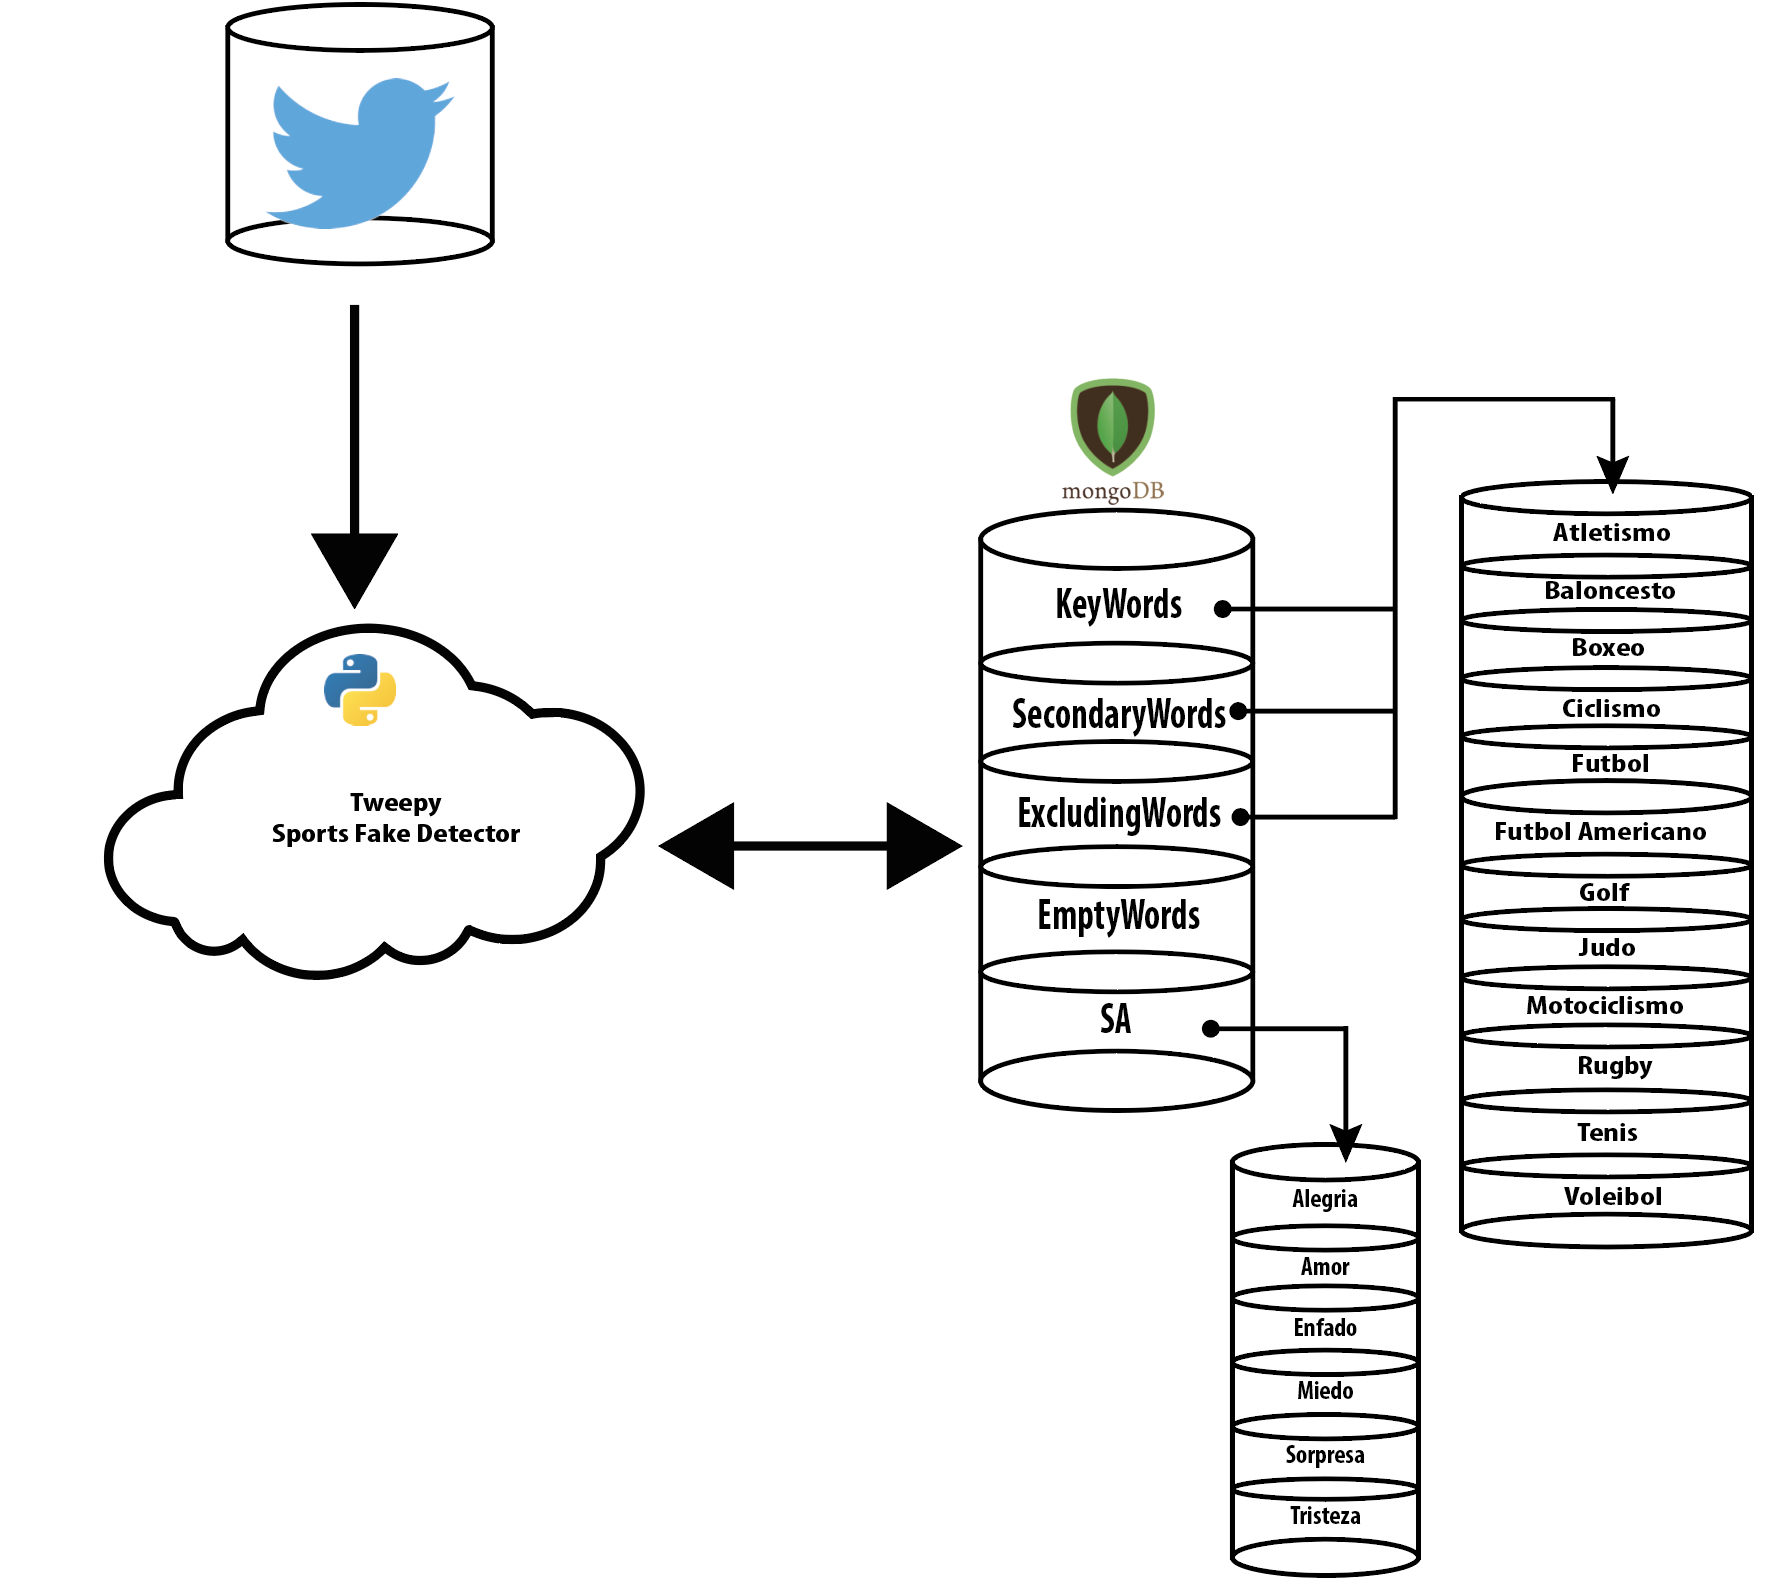
\includegraphics[height=13cm, width=15cm]{imgs/extraccionTwitter.png}
            \caption{Estructura de extracción de tweets y interacción con diccionario}
        \end{figure}
        Donde se puede ver que se extrae la información de twitter a través de la librería tweepy, se proceso con el detector de mentiras y se interacciona con la base de datos donde previamente se habían guardado los diccionarios.\\
        Las tablas de la base de datos son las siguientes:
        \begin{figure}[H]
        \centering
            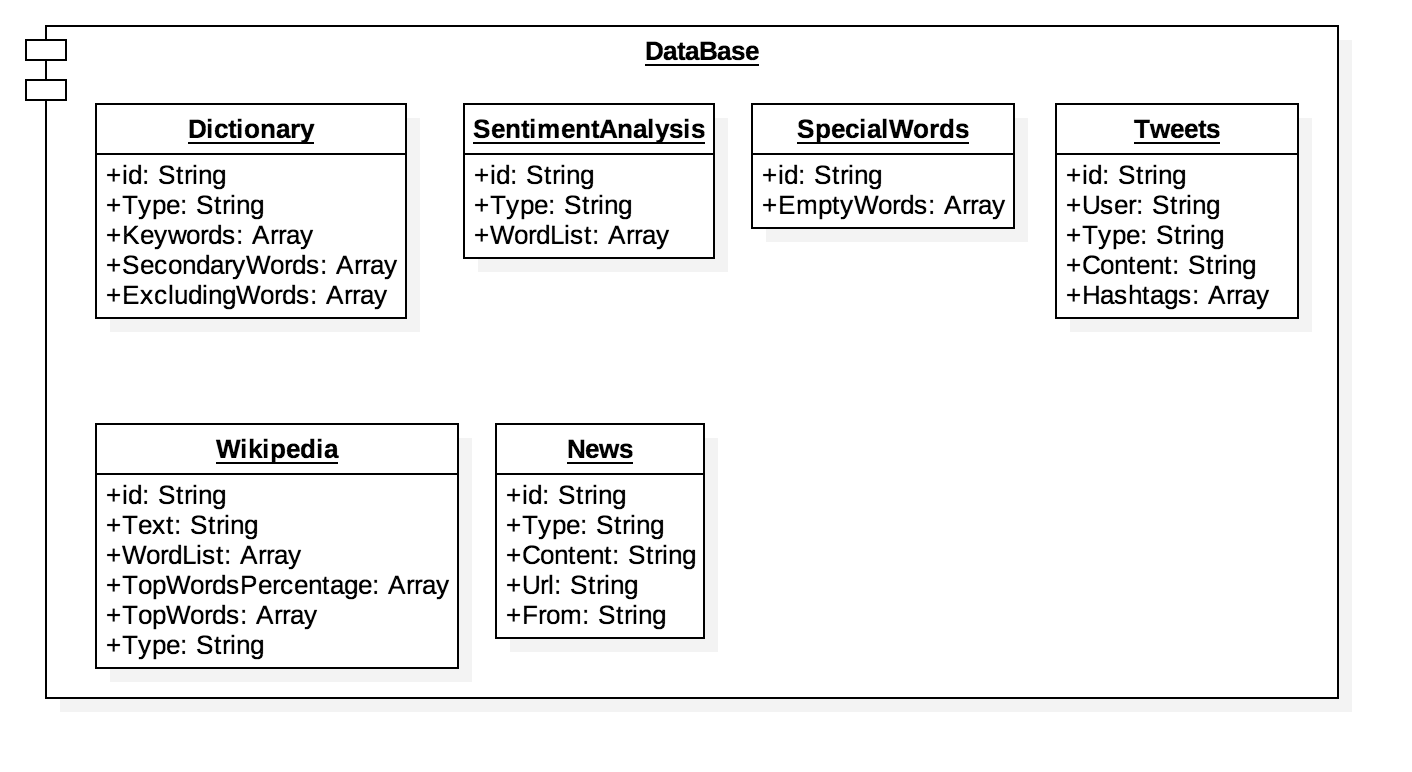
\includegraphics[height=15cm, width=15cm]{imgs/DB.png}
            \caption{Tablas en la base de datos del proyecto}
        \end{figure}
    
        \paragraph{Tweepy 3.5}
            Tweepy es una librería de código abierto para Python que incluye todo el conjunto de funciones necesarias para comunicar con Twitter mediante las API's definidas por este. Las funciones definidas por Tweepy simplifican la conexión y búsquedas con Twitter. Por ejemplo, toda la conexión con Twitter debe estar certificada con un autor y, mientras que por defecto habría que configurar esta conexión mediante otra librería como sería Python-Auth y establecer cada conexión manualmente, Tweepy simplifica esto con unas funciones que simplemente esperan está autenticación como parámetro para poder configurarlo automáticamente. Estos parámetros son 4 tokens necesarios y eb el caso de la búsqueda solo tenemos que indicarle los parámetros que solicita Twitter, toda la complejidad de las conexiones la trata internamente simplificando el trabajo inmensa,ente. Para el proyecto se ha empleado la versión 3.3 de Tweepy.
            \begin{figure}[H]
            	\centering
            	\includegraphics[height=7cm, width=7cm]{imgs/twitter_class.png}
            	\caption{Diagrama de la clase propia Twitter encargada de la comunicación con twitter mediante la librería tweepy}
            \end{figure}
        \paragraph{Wikipedia 1.4.0}
            Está librería se empezó a usar con la finalidad de crear diccionarios automáticamente, simplemente coger todas las palabras que salen de una búsqueda en wikipedia, excluir todos los artículos, proposicionales y palabras que no aportan valor de clasificación.\\
            
            De todas las palabras obtenidas se cogían el 30\% de las palabras más repetidas. Esto permitió empezar a hacer pruebas de los algoritmos pero se descarto por falta de precisión y se empezó a hacer un diccionario propio que ganó riqueza por algunas palabras encontradas gracias a este algoritmo.
            

\newpage    
\subsection{Fase 1 - Clasificación de texto según temática}
    \subsubsection{Concepto}
        {\color{red} 
            TODO
        }
    \subsubsection{Software}
        {\color{red} 
        TODO: Hablar de las librerías python utilizadas, diagrama ...
        }
        \paragraph{Stemmer}
            {\color{red} 
                TODO
            }
        \paragraph{Naive Bayes}
            {\color{red} 
                TODO
            }
        \paragraph{Diccionario}
            {\color{red} 
                TODO
            }

\newpage
\subsection{Fase 2 - Análisis del sentimiento}
    \subsubsection{Concepto}
            {\color{red} 
                TODO
            }
    \subsubsection{Software}
        {\color{red} 
        TODO: Hablar de las librerías python utilizadas, diagrama ...
        }
        \paragraph{Vader Sentiment}
            {\color{red} 
                TODO
            }
        \paragraph{TextBlob}
            {\color{red} 
            Para traducir y para clasificar
            }
        \paragraph{Diccionario}
            {\color{red} 
            Para traducir y para clasificar
            }
\newpage
\subsection{Fase 3 - }
    \subsubsection{Concepto}

    \subsubsection{Software}
\end{document}
